%!TEX root = ./report.tex
\section{Solution}
The provided solution consumes a set of 2D points  $P$ and returns  $D$ for performing point location queries in a Voronoi diagram corresponding to $P$. The attached CD contains the implementation as C\# source code that builds against .NET 4.0. An example providing $P$ and querying $D$ can be found in the program main.  A parser and example for generating data points from  the geographical coordinates of a set of fast-food restaurants is included. 
\paragraph{}
The solution is based on the description provided in \cite{computational_geometry} on point location and Voronoi diagrams, and as such, we do not cover the everything in detail, but rather provide highligts of parts that we found to be tricky to get right.  The implementation of Fortunes algorithm is an open-source implementation that can be found at [cite to misc and codeplex project] . Also , the solution includes a simple GUI from [cise to misc and ref to other os project] that can be useed to visualize simple small-scale datasets.  The implementation of $T$ and $D$ is provided by the authors and our main work constitues in implementing these, besides briding with Fortunes algorithm.
\paragraph{}
One way of accomplishing what we want would be to simply take to the output of Fortunes algorithm, that is, the generated edges, and give them as input to the algorithm for the trapezoidal map. Both algorithms run in O(nlogn)  so the the complexity of running the two in sequence is the same. Alternatively we could add the edges to $T$ on the fly as the are found by Fortunes. It is easy to see that we will get the same complexity as we are virtually doing the same thing. To show this easy connecting of the two algorithms, the implementation demonstrates the latter.

\subsection{Point location in Voronoi}
$D$ is implemented with a standard composite-pattern, and offers a $Find(point)$ operation that will return a bounding trapezoid for the query point.  Recall that a trapezoid is simply defined by its side points and top and bottom segment. And as each segment is just a segment w egot from the Voronoi diagram, it holds a reference to the site of the voronoi cell. Fortunes algorithm adds this edge to site reference, and, eventually, it is the only way that trapezoid can tell which Voronoi cells it lies in. Of course, queies will only be precise when all segments have been added, and all trapezoids are completely trapped inside Voronoi cells.
\paragraph{}
Each time a segment is discovered for the Voronoi diagram, it is inserted into the trapezoidal map, and $T$ is updated with new subtrees according to the new trapezoids that appear from the inserting the new segment. A this point a lot or re-wiring occurs, as new and existing trapezoids need to have their neighbourhoods re-wired correctly. In particular this gets tricky when a new segment crosses several existing trapezoids. \cite{computational_geometry} provides an good description of how to handle this and is depicted in Figure ~\ref{fig:intersecting_segments}. The situation requires that we handle several situations. First of all we need to handle the situation, when one or both of the new segment's endpoints are connected to existing vertices. Secondly, we have to create new trapezoids that are, in some sense, horizontial merges of existing trapezoids. As an example, in  Figure ~\ref{fig:intersecting_segments}, we create  trapezoid $C$ with a left point from Delta 1, a right point that will be the right most vertex of the newly inserted segment, top being the new segment too, and bottom being the the segment shared by  Delta 1,  Delta 2 and  Delta 3.   

\begin{figure}[t]
    \centering
      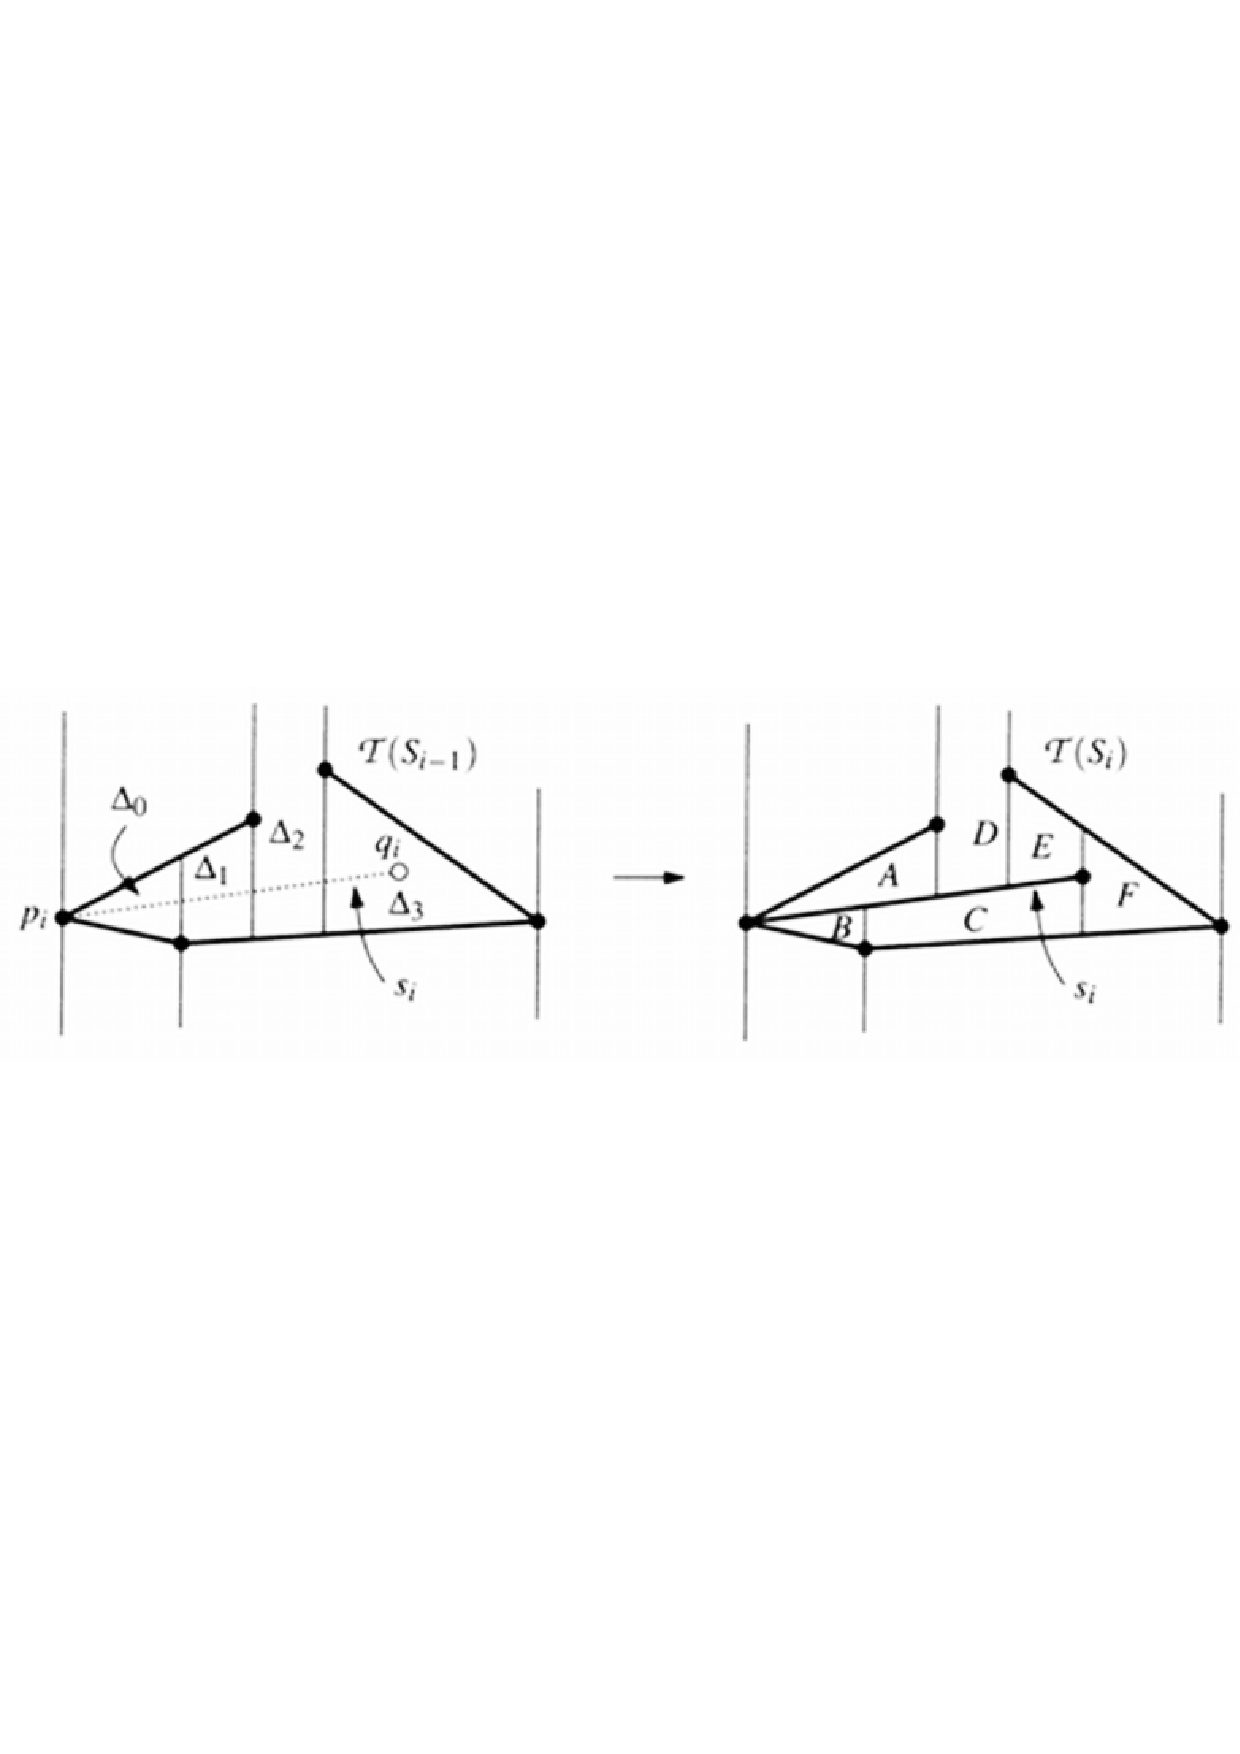
\includegraphics[height=80mm]{images/intersecting_segments.pdf}
    \caption{Inserting a segment that crosses several trapezoids}
    \label{fig:intersecting_segments}
\end{figure}


%Explain merge of cells situation, and maybe provide pseudo code of how we did it.
%Discuss implementaion dificulties, like updating neighbours, unprecise doubles in search tree.
%Porlbmees with voronoi implemenation, stuff that probably doesnt work with real fast food restaurant data set.

\subsection{Expected Customers}
%Expected number of hits by random shooting of points on the map. Chernoff expectation vs size of voron oi cells.

